\documentclass[twoside,11pt]{article}

% Any additional packages needed should be included after jmlr2e.
% Note that jmlr2e.sty includes epsfig, amssymb, natbib and graphicx,
% and defines many common macros, such as 'proof' and 'example'.
%
% It also sets the bibliographystyle to plainnat; for more information on
% natbib citation styles, see the natbib documentation, a copy of which
% is archived at http://www.jmlr.org/format/natbib.pdf

\usepackage{jmlr2e}
\usepackage[T1]{fontenc}

% Additional packages
\usepackage{booktabs}         % for \toprule, \midrule, \bottomrule
\usepackage{threeparttable}   % for threeparttable + tablenotes
\usepackage{amsmath}
\usepackage{amsfonts}
\usepackage{amssymb}
\usepackage{array}
\usepackage{multirow}
\usepackage{longtable}
\usepackage{xurl}
\usepackage{subcaption}
% \usepackage{float} removed: [H] specifier is prohibited by JMLR style

% Definitions of handy macros can go here
\newcommand{\dataset}{{\cal D}}
\newcommand{\fracpartial}[2]{\frac{\partial #1}{\partial  #2}}

% Heading arguments are {volume}{year}{pages}{date submitted}{date published}{paper id}{author-full-names}
\usepackage{lastpage}
\jmlrheading{XX}{2025}{1-\pageref{LastPage}}{XX/XX}{XX/XX}{XX-XXXX}{Tinashe Ngorima}

% Short headings should be running head and authors last names
\ShortHeadings{Evaluating Chatterjee’s \(\xi_n\) for Feature Selection}{Ngorima}
\firstpageno{1}

\begin{document}

\title{Evaluating Chatterjee’s \(\xi_n\)
for Feature Selection in Critical Temperature Prediction  }

\author{\name Tinashe Ngorima \email tngorima@su.edu.om \\
       \addr General Foundation Program\\
       Sohar University\\
       Sohar, Oman}

% Editor field left blank for initial submission
\editor{}

\maketitle

%%%%%%%%%%%%%%%%%%%%%%%%%%%%%%%%%%%%%%%%%%%%%%%%%%%%%%%%%%
% ABSTRACT 
%%%%%%%%%%%%%%%%%%%%%%%%%%%%%%%%%%%%%%%%%%%%%%%%%%%%%%%%%%
\begin{abstract}%

\end{abstract}
\begin{abstract}%
High-dimensional scientific datasets often exhibit redundancy and nonlinear dependence, motivating feature selection methods that balance predictive performance, computational efficiency, and stability. We present a systematic evaluation of Chatterjee’s $\xi_n$ as a filter-based feature selection criterion, compared against mutual information (MI), maximal information coefficient (MIC), and distance correlation (DC), on a superconductivity dataset with 15,542 samples and 81 descriptors.

Evaluation is conducted across 48 feature-selection configurations and 30 repeated resamplings per configuration. To ensure robust assessment, we adopt a layered inferential framework in which Friedman tests assess global rank differences, Nemenyi post-hoc analysis identifies pairwise contrasts, Cohen's $d_z$ quantifies effect sizes, BCa bootstrap confidence intervals estimate uncertainty, and Jaccard similarity measures feature-selection stability.

DC achieves the highest predictive performance ($R^2 = 0.893 \pm 0.010$), followed by MI and MIC, while $\xi_n$ reaches 94\% of peak performance with strong stability (Jaccard $= 0.95 \pm 0.06$) and a 5.6$\times$ computational advantage at 20\% feature retention. Friedman testing confirms significant rank differences (DC $\succ$ MI $\approx$ MIC $\succ$ $\xi_n$). Despite a 6\% performance gap relative to DC, $\xi_n$ exhibits the lowest generalization gap ($\Delta R^2 = 0.031 \pm 0.007$), indicating strong overfitting resistance.

Overall, results characterize the accuracy--stability--efficiency trade-off of $\xi_n$ under controlled benchmarking, isolating methodological effects from domain variability.
\end{abstract}

\begin{keywords}
benchmarking, feature selection, high-dimensional data, rank correlation,
regression, stability analysis
\end{keywords}

%%%%%%%%%%%%%%%%%%%%%%%%%%%%%%%%%%%%%%%%%%%%%%%%%%%%%%%%%%
\section{Introduction}
%%%%%%%%%%%%%%%%%%%%%%%%%%%%%%%%%%%%%%%%%%%%%%%%%%%%%%%%%%
Machine learning applications in scientific domains increasingly operate on
high-dimensional datasets characterized not only by large feature spaces but
also by substantial multicollinearity, redundancy, and noise. Superconductivity
research exemplifies this regime, where predicting the critical temperature
$T_c$ from compositional descriptors is a central problem with implications for
quantum materials discovery, energy-efficient power transmission, and medical
imaging \citep{Stanev2018machine}. The dataset introduced by
\citet{Hamidieh2018data} and later curated by \citet{Matasov2020vis}
(81 descriptors, 21,263 samples) exhibits operational high dimensionality through
correlated descriptors, sparsity, and heavy-tailed variability. In such settings,
feature selection is not merely a computational convenience but a prerequisite
for stable and interpretable learning.

A wide range of dependence measures have been proposed for filter-based feature
selection. Classical approaches such as Pearson's correlation \citep{Pearson1900},
Spearman's $\rho$ \citep{Spearman1904}, and Kendall's $\tau$ \citep{Kendall1938}
are computationally efficient but limited to linear or monotonic relationships.
More recent methods, including mutual information (MI) \citep{Ross2014mutual},
the maximal information coefficient (MIC) \citep{Reshef2011}, and distance
correlation (DC) \citep{Szekely2007}, extend this capability to nonlinear
dependence. However, these methods introduce practical trade-offs: MI requires
density estimation and is sensitive to discretization; MIC involves adaptive
grid-search procedures with nontrivial computational overhead; and DC, while
consistent, incurs quadratic complexity in sample size. Consequently, their
suitability as scalable and stable feature ranking criteria in high-dimensional
scientific settings remains context-dependent.

Chatterjee's rank correlation coefficient $\xi_n$ \citep{Chatterjee2021} has
recently emerged as a theoretically principled nonparametric measure of dependence
that detects general functional relationships while retaining a simple rank-based
formulation and bounded, interpretable range ($\xi_n \in [0,1]$). A key
distinction of $\xi_n$ lies in its asymmetric construction: whereas MI, MIC,
and DC quantify mutual dependence symmetrically, $\xi_n$ estimates the extent
to which one variable is a measurable function of another through order
statistics. This yields two practically important properties: (i)~invariance to
strictly monotonic transformations of the response, and (ii)~sensitivity to
directional functional relationships that symmetric criteria may not capture.
These properties may be advantageous in feature selection settings where
predictors are ranked with respect to a response variable. Despite these 
conceptual advantages, the empirical behavior of $\xi_n$ in high-dimensional 
feature selection pipelines—particularly under resampling and stability 
constraints—remains largely unexplored.

Existing studies evaluate dependence measures primarily in
terms of detection power or asymptotic properties, but provide little evidence
on their behavior as feature ranking criteria within realistic, resampling-based
learning pipelines. In particular, the accuracy--stability--robustness trade-offs
of $\xi_n$ relative to established nonlinear measures remain uncharacterized,
limiting its principled adoption in practice.

In this work, we address this gap by systematically evaluating $\xi_n$ as a
filter-based feature selection criterion against MI, MIC, and DC on a standard
materials-informatics benchmark. The study is designed to isolate the effect of
dependence estimation on downstream predictive performance by controlling for
model class and data variability through repeated experiments and nonparametric
statistical validation. The central research question is:

\begin{quote}
\emph{How does $\xi_n$ compare to modern dependence measures as a feature
ranking criterion in high-dimensional scientific data, when evaluated jointly
in terms of predictive accuracy, selection stability, and robustness under
resampling?}
\end{quote}

This work makes the following contributions:

\begin{enumerate}

  \item  
  We provide a comparative empirical evaluation of $\xi_n$ as a
  filter-based feature ranking criterion, benchmarked against MI, MIC, and DC
  across 48 experimental configurations on a canonical superconductivity dataset.

  \item
  This study moves beyond single-metric evaluation by quantifying trade-offs between
  predictive performance ($R^2$), selection stability (Jaccard similarity),
  and variability (coefficient of variation) using 30-repetition resampling
  experiments and nonparametric statistical testing.

  \item
  The results shoe that while DC achieves the highest predictive accuracy,
  $\xi_n$ attains comparable stability with only a modest performance gap
  (6\% in $R^2$) and the smallest generalization gap of all four methods,
  revealing a trade-off that is not captured by existing evaluations of
  dependence measures.

  \item 
  We provide empirically anchored selection guidelines for dependence measures
  in filter-based feature selection under competing constraints of accuracy,
  stability, and computational budget.

\end{enumerate}

The experiment is restricted to a single domain to isolate accuracy--stability
trade-offs from domain-transfer confounds. This methodological choice enables
clean attribution of observed performance differences to the ranking quality of
each dependence measure.

%%%%%%%%%%%%%%%%%%%%%%%%%%%%%%%%%%%%%%%%%%%%%%%%%%%%%%%%%%
\section{Related Work}
%%%%%%%%%%%%%%%%%%%%%%%%%%%%%%%%%%%%%%%%%%%%%%%%%%%%%%%%%%
We organize the prior literature along three axes that directly motivate 
this study: statistical foundations of filter-based feature selection 
(\S\ref{sec:stat-foundations}), scalability and data-quality constraints 
governing method applicability (\S\ref{sec:scalability}), and stability 
and reproducibility frameworks used to assess dependence measures 
(\S\ref{sec:stability}). Taken together, these strands reveal that no 
existing benchmark jointly characterizes $\xi_n$, DC, MI, and MIC under 
a unified accuracy--stability--robustness protocol on complex 
scientific data.

\subsection{Statistical Foundations of Feature Selection}
\label{sec:stat-foundations}
High-dimensional regression ($p \gg n$) raises a trilemma between predictive
accuracy, scalability, and stability \citep{Venkatesh2023}. Feature selection
methods address this by reducing dimensionality before or during model fitting.
Among these, filter methods are especially prominent in scientific applications
where interpretability and computational efficiency are critical
\citep{Guyon2003intro}.

Formally, a filter is a scoring operator
\[
\mathcal{S} : \mathbb{R}^{n \times p} \times \mathbb{R}^{n} \to \mathbb{R}^{p},
\quad \mathcal{S}_{j} = \phi(X_{j},\, y),
\]
where $\phi$ is a dependence measure that ideally satisfies consistency
($\phi = 0 \iff X_{j} \perp y$), $\sqrt{n}$-estimability, and computational
tractability. A critical distinction among dependence measures is symmetry.
Classical coefficients (Pearson, Spearman, Kendall) and modern symmetric
measures (DC, MI, MIC) satisfy $\phi(X, Y) = \phi(Y, X)$, quantifying
bidirectional association. In contrast, Chatterjee's $\xi_n$ is asymmetric.
$\xi_n(X, Y)$ quantifies the functional dependence of $Y$ on $X$ through
nearest-neighbour ranks, measuring how well $X$ predicts $Y$ rather than their
mutual association \citep{Chatterjee2021}. For feature selection, this
directional property is advantageous: it scores each feature's predictive
contribution to the target while avoiding inflation from reverse dependencies
that symmetric measures capture.

Early comparative work on nonlinear dependence measures has established that MI
is widely used due to its information-theoretic generality, but practical
implementations require density estimation or discretization, introducing bias
and sensitivity to hyperparameters \citep{Ross2014mutual}. MIC was introduced
to provide equitability across functional relationships, but its adaptive grid
search results in substantial computational overhead \citep{Reshef2011}. DC
offers a consistent test of independence and has been successfully applied in
feature screening, although its quadratic complexity in sample size limits
scalability \citep{Szekely2007}. $\xi_n$ \citep{Chatterjee2021} has recently
been introduced with strong theoretical guarantees, including consistency
against all alternatives. Table~\ref{tab:char} summarizes the key operational
properties of the four methods.

\begin{table}[t]
\centering
\caption{Key properties of the four correlation-based feature selection methods.}
\label{tab:char}
\begin{tabular}{lccccc}
\toprule
Method & Nonlinear & Symmetric & Binning & Outlier Sensitivity & Complexity \\
\midrule
$\xi_n$ & Yes & No  & No       & Low      & $\mathcal{O}(n \log n)$ \\
MI      & Yes & Yes & Yes      & High     & $\mathcal{O}(n \log n)$ \\
MIC     & Yes & Yes & Adaptive & High     & $\mathcal{O}(n^{1.2})$  \\
DC      & Yes & Yes & No       & Moderate & $\mathcal{O}(n^{2})$    \\
\bottomrule
\end{tabular}
\end{table}

\subsection{Scalability and Data Quality Challenges}
\label{sec:scalability}
Scientific datasets often combine large sample sizes with sparsity and
heavy-tailed noise \citep{Matasov2020vis}. Rank-based dependence measures such
as $\xi_n$ are less distorted by sparsity artifacts that inflate MI and MIC
scores through the Laplace correction \citep{Fernandes2010, Frenay2013,
Cao2021}. The $\mathcal{O}(n \log n)$ complexity of $\xi_n$ also positions it
favorably against DC's $\mathcal{O}(n^2)$ as sample sizes grow, though the
empirical crossover point depends on the $(n,u\, p)$ scaling regime and
domain-specific correlation structure.

\subsection{Stability and Reproducibility}
\label{sec:stability}
Feature selection must deliver stable rankings across resamples, because
stability directly affects reproducibility in downstream validation
\citep{Buyukkececi2023review}. Chatterjee's coefficient admits
distribution-free asymptotic variance estimates \citep{Shi2022biometrika},
generating more consistent feature rankings. Beyond algorithmic stability,
recent work has emphasized stability-based evaluation frameworks that assess the
reproducibility of selected feature subsets under data perturbations, using
resampling techniques and similarity metrics such as the Jaccard index
\citep{Nogueira2016jaccard}. However, most such studies focus on algorithmic
selection methods (e.g., LASSO, tree-based models) rather than on the
dependence measures underlying filter-based ranking.

Despite growing interest in nonlinear correlation measures, comparative evaluations jointly evaluating DC, MI, MIC, and $\xi_n$ unified accuracy--stability--robustness protocols remain limited. The present work addresses this gap.

\paragraph{Formal Problem Definition.}
Let $\mathcal{D} = \{(x_i, y_i)\}_{i=1}^n$ denote a dataset with response
variable $y \in \mathbb{R}$ and feature matrix $X \in \mathbb{R}^{n \times p}$,
where $p$ may be large and features exhibit substantial redundancy and
dependence. Let $\mathcal{M} = \{m_1, \dots, m_K\}$ denote a set of dependence
measures, where each $m_k$ induces a ranking function
$r_k : \{1, \dots, p\} \to \mathbb{R}$ based on pairwise dependence between
each feature and the response. For a given retention level $\alpha \in (0,1]$,
let $S_k^{(\alpha)} \subseteq \{1, \dots, p\}$ denote the subset of top-ranked
features selected by $m_k$. We study the problem of selecting a dependence
measure $m_k$ that optimizes feature selection performance under three criteria:
(i)~predictive accuracy, measured by the generalization performance of a
downstream regression model trained on $S_k^{(\alpha)}$;
(ii)~selection stability, quantified by the consistency of $S_k^{(\alpha)}$
under repeated resampling of $\mathcal{D}$; and
(iii)~robustness, defined as the variability of predictive performance across
resampling trials. The objective is to characterize the trade-offs between these
criteria across $m_k \in \mathcal{M}$, and in particular to evaluate the
behavior of $\xi_n$ \citep{Chatterjee2021} relative to established dependence
measures in high-dimensional scientific data.

%%%%%%%%%%%%%%%%%%%%%%%%%%%%%%%%%%%%%%%%%%%%%%%%%%%%%%%%%%
\section{Methods}
%%%%%%%%%%%%%%%%%%%%%%%%%%%%%%%%%%%%%%%%%%%%%%%%%%%%%%%%%%
To isolate methodological effects from domain-specific confounding, the study
is intentionally restricted to a single application domain. This design choice
enables a controlled comparison in which observed differences can be attributed
directly to the ranking behavior of each dependence measure rather than to
cross-domain variability.

\subsection{Experimental Pipeline}
We formalize the feature selection and prediction workflow as a structured
pipeline consisting of three sequential components: (i)~dependence-based feature
ranking, (ii)~threshold-based subset selection, and (iii)~downstream supervised
learning.

Let $\mathcal{D} = \{(x_i, y_i)\}_{i=1}^n$ denote the dataset with feature
matrix $X \in \mathbb{R}^{n \times p}$ and response variable $y \in \mathbb{R}$.
For each dependence measure
$m \in \mathcal{M} = \{\xi_n,\, \mathrm{MI},\, \mathrm{MIC},\, \mathrm{DC}\}$,
we compute a score vector
\[
s_m = [s_m(x_1, y), \dots, s_m(x_p, y)],
\]
which induces a ranking function $r_m$ ordering features in decreasing dependence
with respect to $y$.

\textit{Feature Ranking Step.} Each method $m$ assigns a scalar dependence score to every feature individually.
Scores are computed on the training partition only to prevent information leakage.
The resulting ranking $r_m$ is used as the sole criterion for feature selection,
ensuring that all downstream differences arise exclusively from the dependence
measure.

\textit{Selection Threshold $\alpha$.} Given a retention level $\alpha \in \{0.10, 0.15, 0.20\}$, we define the
selected feature subset as
\[
S_m^{(\alpha)} = \text{Top-}\lfloor \alpha p \rfloor \text{ features under }
r_m.
\]
This fixed-percentage strategy ensures comparability across methods by
controlling for dimensionality effects and isolating the influence of ranking
quality on model performance. The chosen range (10\%--20\%) reflects
empirically validated optimal regimes for superconductivity prediction tasks
in prior studies \citep{Stanev2018machine, Matasov2020vis}.

\textit{Regression Models.} To evaluate the predictive utility of each selected subset $S_m^{(\alpha)}$,
we consider four regression models spanning linear and nonlinear learning
paradigms: Lasso \citep{Tibshirani1996lasso}, Elastic Net
\citep{ZouHastie2005elasticnet}, LightGBM \citep{Ke2017lightgbm}, and Random
Forest \citep{Breiman2001rf}. This heterogeneous model class design ensures that
observed performance differences among feature selection methods are attributable
to the ranking strategy rather than model-specific bias
\citep{Boulesteix2013plea, Munozpreto2022}.

\subsection{Dataset and Data Quality Assessment}
\label{sec:dataset}
The superconductivity dataset \citep{Hamidieh2018data, Matasov2020vis} is
selected as the benchmark for four criteria: (i)~a sufficiently large feature
space to exhibit operational high dimensionality; (ii)~pronounced
multicollinearity and redundancy, which stress-test dependence estimators under
correlated and noisy inputs; (iii)~a continuous regression target ($T_c$),
enabling evaluation via standard predictive metrics ($R^2$, RMSE, MAE); and
(iv)~established use in prior materials informatics studies, ensuring
comparability with existing literature
\citep{Stanev2018machine, Yu2023prediction, Carral2024interpretably}.

We adopt an operational definition of high dimensionality: a dataset is
\emph{operationally high-dimensional} if feature redundancy and multicollinearity
are sufficiently severe to affect dependence estimation and ranking stability,
regardless of whether the classical condition $p \gg n$ holds. This definition
is consistent with conventions in materials informatics, where
moderate-dimensional descriptor spaces ($p \approx 80$) can still induce strong
collinearity and sparsity effects that motivate dimensionality reduction
\citep{Fan2014challenges, Johnstone2009statistical, Stanev2018machine,
Yu2023prediction}.

The curated dataset contains $n = 15{,}542$ observations after removal of
approximately 6,000 duplicates from the original 21,263-sample corpus
\citep{Hamidieh2018data}. Each observation is described by 81 features
(78 continuous and 3 integer-valued descriptors), with critical temperature
$T_c$ as the response variable. The feature set is constructed from eight
elemental atomic properties combined with ten statistical aggregation functions,
yielding $8 \times 10 = 80$ engineered descriptors plus one stoichiometric
fraction feature. This construction induces substantial redundancy, reflected in
a condition index exceeding 30 for more than half (52\%) of the features.
Additional diagnostics indicate widespread sparsity (zeros in 48 features,
59.3\%) and substantial outlier prevalence (IQR-based outliers in 67 features,
82.7\%, with 15 features exceeding a 10\% outlier rate).

Stratified random sampling partitions the data into training (64\%,
$n = 9{,}947$), validation (16\%, $n = 2{,}487$), and test (20\%,
$n = 3{,}108$) sets. Stratification preserves the empirical distribution of
$T_c$ across all splits.

\subsection{Feature Selection}
Feature selection is formulated as a dependence-driven ranking problem in which
each method induces a total ordering of features with respect to the target
variable $T_c$. For each method
$m \in \{\xi_n,\, \mathrm{MI},\, \mathrm{MIC},\, \mathrm{DC}\}$, a feature
ranking $r_m$ is computed on the training data only. The top-ranked features
are then selected according to a fixed retention level $\alpha$, yielding a
subset $S_m^{(\alpha)}$. This design ensures that all downstream differences in
predictive performance and stability are attributable solely to the ranking
induced by $m$.

Feature retention thresholds of 10\% (8 features), 15\% (12 features), and
20\% (16 features) align with the empirically established optimum for
critical-temperature prediction. \citet{Stanev2018machine} and
\citet{Matasov2020vis} identify approximately 17 features as optimal, closely
matching our 20\% threshold, and the broader literature indicates 6 to 29
features as the effective range (Table~\ref{tab:superconductivity-benchmark}).
The three thresholds produce 12 distinct feature selection configurations per
experimental repetition, enabling controlled comparison of ranking stability and
predictive performance across dependence measures.

\begin{table}[t]
\centering
\caption{Prediction accuracy across representative studies on critical
temperature prediction tasks.}
\label{tab:superconductivity-benchmark}
\begin{tabular}{lcccc}
\toprule
\textbf{Study} & \textbf{Features} & $\boldsymbol{R^{2}}$
  & $\boldsymbol{\mathrm{MAE}\,(\mathrm{K})}$
  & $\boldsymbol{\mathrm{RMSE}\,(\mathrm{K})}$ \\
\midrule
\text{This work (DC--LightGBM)} & 16 (20\%) & \text{0.881}
  & \text{7.16} & \text{11.51} \\
\citet{Hamidieh2018predict} & 81 (100\%) & 0.920 & 9.50 & 17.40 \\
\citet{GarciaNieto2021prediction} & 15--20 & 0.915 & 5.80 & --- \\
\citet{Yu2023prediction} & 29 & 0.931 & 7.21 & 9.82 \\
\citet{Carral2024interpretably} & 6 & --- & 5.19 & --- \\
\bottomrule
\end{tabular}
\smallskip\\
{\small\textit{Note.} Benchmark values for prior studies were extracted from the
corresponding published articles. The proposed model attains competitive
predictive accuracy using only 20\% of the original descriptor set.}
\end{table}

Feature ranking and subset construction are performed using the training split
only, after which the selected feature columns are applied unchanged to the
validation and test splits to prevent feature selection leakage. In particular,
\citet{Carral2024interpretably} obtained the lowest MAE in the literature using
only 6 descriptors, confirming that aggressive dimensionality reduction is
viable on this dataset.

\subsection{Model Implementation and Evaluation}
The objective of the evaluation stage is to assess how effectively different
dependence-based feature ranking methods induce subsets that support accurate,
stable, and generalizable prediction. The learning algorithms serve as downstream
evaluators of feature subset quality rather than as objects of study.

Lasso \citep{Tibshirani1996lasso} and Elastic Net
\citep{ZouHastie2005elasticnet} enforce $\ell_1$ and combined $\ell_1$/$\ell_2$
regularization, respectively, providing interpretable linear baselines under
multicollinearity \citep{Hastie2019}. LightGBM \citep{Ke2017lightgbm} and
Random Forest \citep{Breiman2001rf} capture nonlinear feature interactions
through gradient boosting and bootstrap aggregation, respectively
\citep{Grinsztajn2022tree}. This heterogeneous design ensures that observed
performance differences across feature selection methods are attributable to
ranking quality rather than model-specific inductive bias.

All preprocessing steps, including standardization, are performed within a
\texttt{scikit-learn} pipeline and recomputed independently within each
cross-validation fold. Scaling parameters are estimated strictly from the
fold-specific training partition. Feature scores are computed exclusively on
the training data, and the resulting subset $S_m^{(\alpha)}$ is transferred
unchanged to the validation and test partitions without recomputation or
refitting. This strict separation ensures that feature selection, scaling, and
model fitting are fully decoupled across data partitions, preventing all forms
of information leakage.

Hyperparameter optimization is performed using Bayesian optimization via Optuna,
with 50 trials per model in Experiment~1 and 20 trials in Experiment~2. A
5-fold cross-validation procedure is applied within the training data to estimate
generalization performance during tuning. Final model evaluation is conducted
exclusively on the independent test set, which is never accessed during feature
selection or hyperparameter optimization.

Predictive performance is measured using $R^2$, RMSE, and MAE. In addition, the
generalization gap
\[
\Delta R^2 = R^2_{\text{train}} - R^2_{\text{test}}
\]
is used as an indicator of overfitting sensitivity induced by different feature
ranking methods.

\subsection{Experimental Design}
The experimental design is structured to evaluate both (i)~the comparative
predictive performance of dependence-based feature ranking methods and
(ii)~the stability of induced feature subsets under resampling variability.

\subsubsection{Experiment~1: Comprehensive performance evaluation (48 configurations).}
All combinations of 4 feature selection methods $\times$ 3 retention thresholds
$\times$ 4 regression models are evaluated, resulting in 48 configurations.
A single train--test split (\texttt{RANDOM\_SEED}$= 53$; pipeline
\texttt{random\_state}$= 42$ for cross-validation and model initialization) is
used to establish baseline performance rankings and identify the optimal
method--model combination. The goal of this experiment is controlled comparison
of ranking quality across methods under identical modeling conditions.

\subsubsection{Experiment~2: Stability and reproducibility analysis (30 repetitions).}
To quantify the robustness of feature ranking methods, we conduct 30 independent
repetitions of the full pipeline using distinct train--test splits
$r \in \{0, 1, \ldots, 29\}$ (80\%--20\% partitioning). For each repetition,
feature selection is performed exclusively on the training split, followed by
hyperparameter tuning via Optuna (20 trials) and evaluation on the held-out
test set. The \texttt{random\_state}$= 42$ is fixed for LightGBM, Optuna, and
\texttt{mutual\_info\_regression} across all repetitions. Stability is quantified
using pairwise Jaccard similarity computed over all $\binom{30}{2} = 435$
pairwise comparisons of selected feature subsets per method. Complete seed
assignments and package versions are recorded in \texttt{requirements.txt} in
the accompanying repository
(DOI: \href{https://doi.org/10.5281/zenodo.19675804}{10.5281/zenodo.19675804}).

\subsection{Statistical Validation}
Overall differences in predictive performance are assessed using the Friedman
test \citep{Friedman1937ranks, Demvsar2006}, a nonparametric test for multiple
related samples that evaluates the null hypothesis that all methods perform
equivalently in terms of their average rank across repeated experimental
conditions. When the Friedman test indicates statistically significant
differences, pairwise comparisons are conducted using the Nemenyi post-hoc
test \citep{Demvsar2006}, which identifies groups of methods whose average ranks
are not significantly different.

Selection stability is evaluated from multiple complementary perspectives.
Subset consistency across resampling runs is quantified using the Jaccard
similarity coefficient \citep{Nogueira2016jaccard}, computed over all pairwise
comparisons of selected feature subsets. Variability in predictive performance
across repetitions is quantified using the coefficient of variation (CoV),
capturing sensitivity to sampling noise. Pareto frontier analysis identifies
methods achieving optimal trade-offs between predictive accuracy and stability
without requiring scalarization of objectives.

Complementing the rank-based and stability analyses, pairwise effect sizes
for the 30-repetition experiments are reported as Cohen's paired
$d_z = \bar{\Delta} / s_{\Delta}$, where
$\bar{\Delta}$ and $s_{\Delta}$ are the mean and standard deviation of the
within-pair performance difference across the $n = 30$ shared splits
\citep{Cohen1988, Lakens2013}. Sign convention: $d_z > 0$ indicates that the
row method outperforms the column method on $R^{2}$ (primary metric);
direction is reversed for MAE so that $d_z > 0$ likewise denotes superiority.
Ninety-five percent bias-corrected and accelerated (BCa) bootstrap intervals
are obtained with $B = 10{,}000$ paired resamples (seed
\texttt{20260512}) to accommodate potential bias and asymmetry in
repeated-measures effect-size distributions. Because
$d_z$ is a within-subjects effect size, Cohen's qualitative bands
($0.2 / 0.5 / 0.8$) calibrated for between-subjects $d$ do not transfer
\citep{Lakens2013}; interpretation is therefore anchored on $\bar{\Delta}$ in
$R^{2}$ (or MAE) units, paired with the BCa interval, rather than on a
categorical magnitude label.

%%%%%%%%%%%%%%%%%%%%%%%%%%%%%%%%%%%%%%%%%%%%%%%%%%%%%%%%%%
\section{Results}
%%%%%%%%%%%%%%%%%%%%%%%%%%%%%%%%%%%%%%%%%%%%%%%%%%%%%%%%%%
This section presents comparative performance results, statistical validation, and stability analyses across the evaluated dependence measures.

\subsection{Comprehensive Model Comparison}

Table~\ref{tab:overall_results} summarizes predictive performance across 48 feature-selection configurations and three regression families. Across all settings, tree-based models (LightGBM and Random Forest) consistently outperform linear models, confirming the presence of nonlinear structure in the target variable.

Among feature selection methods, DC achieves the highest predictive performance across nearly all configurations, with MI and MIC exhibiting closely aligned behavior. The $\xi_n$ method consistently yields lower absolute $R^{2}$ values but maintains competitive performance relative to its substantial computational advantage, particularly at the 20\% retention threshold.

Importantly, performance differences are sensitive to the feature retention regime, with the 20\% threshold providing the most stable trade-off between predictive accuracy and model variance across all methods.

\begin{table}[tp]
\centering
\caption{Predictive performance across models and feature selection methods}
\label{tab:overall_results}
\small
\begin{tabular}{@{}llccccc@{}}
\toprule
Model & Method & Threshold & Test $R^2$ & Test RMSE & Test MAE
  & CV RMSE (K) \\
\midrule
\multicolumn{7}{l}{\textit{LightGBM}} \\
LightGBM & DC$^{*}$       & 20\% & \textbf{0.881} & \textbf{11.51} & \textbf{7.16} & 11.21 \\
LightGBM & DC       & 10\% & 0.866 & 12.21 & 7.76 & 12.36 \\
LightGBM & MI       & 20\% & 0.878 & 11.64 & 7.15 & 11.29 \\
LightGBM & MIC      & 20\% & 0.866 & 12.19 & 7.58 & 11.90 \\
LightGBM & $\xi_n$  & 20\% & 0.826 & 13.89 & 8.74 & 13.64 \\
\midrule
\multicolumn{7}{l}{\textit{Random Forest}} \\
RF & DC       & 15\% & 0.808 & 14.59 & 9.60 & 14.34 \\
RF & MI       & 20\% & \underline{0.818} & 14.22 & 9.34 & 13.72 \\
RF & MIC      & 20\% & \textbf{0.818} & \textbf{14.21} & \textbf{9.29} & 14.18 \\
RF & $\xi_n$  & 20\% & 0.790 & 15.28 & 10.26 & 15.11 \\
\midrule
\multicolumn{7}{l}{\textit{Linear models}} \\
Lasso       & DC      & 20\% & 0.599 & 21.12 & 16.07 & 21.16 \\
Lasso       & $\xi_n$ & 20\% & 0.552 & 22.30 & 17.80 & 22.31 \\
Elastic Net & DC      & 20\% & 0.599 & 21.12 & 16.07 & 21.16 \\
\bottomrule
\end{tabular}
\smallskip\\
{\small\textit{Note.} Bold indicates the best result within each model class. The asterisk (*) denotes the overall best-performing method based on average rank across all 48 configurations. CV-RMSE: cross-validated RMSE on the 5-fold training partition and K is kelvin}
\end{table}

\subsection{Statistical Performance Comparison}

To assess whether observed performance differences are statistically robust, we apply a layered inferential framework across the 48 configurations.

The Friedman test reveals significant differences among dependence measures ($\chi^{2} = 27.9$, $p < 0.001$ for $R^{2}$), indicating that at least one method differs in ranking behavior. Post-hoc Nemenyi analysis confirms a consistent ranking structure: DC $\succ$ MI $\approx$ MIC $\succ$ $\xi_n$, with statistically significant separation between DC and all other methods.

To complement rank-based inference, Cohen's $d_z$ is used to quantify paired effect sizes across identical resampling runs. All observed effects are statistically detectable but fall within the negligible-to-small range in standardized terms, indicating that rank separation does not translate into large effect magnitudes.

BCa bootstrap confidence intervals further confirm that effect estimates are stable under resampling, with intervals tightly concentrated around small but consistent differences.

Overall, statistical inference confirms a stable ranking structure while indicating that absolute performance differences are modest in magnitude.

\begin{figure}[t]
\centering
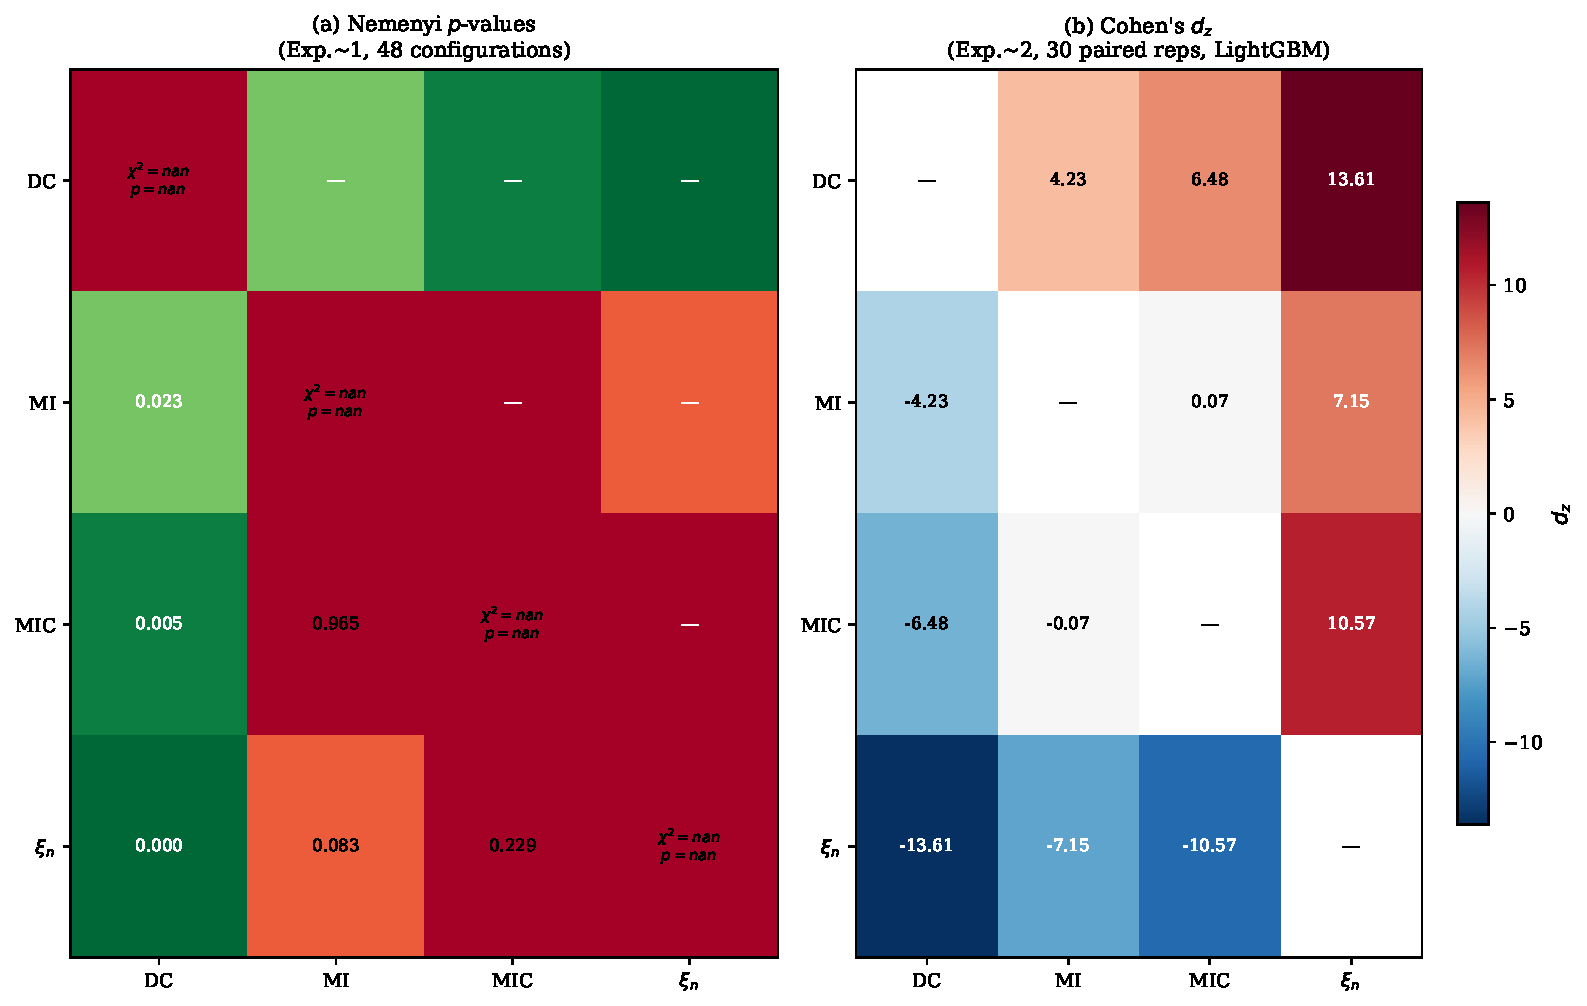
\includegraphics[width=\columnwidth]{fig1_stat_tests}
\caption{Statistical inference across 48 experimental configurations.
\textbf{(a)}~Nemenyi post-hoc adjusted $p$-values ($R^{2}$ metric).
Diagonal: Friedman $\chi^{2} = 27.9$, $p < 0.001$.
Lower triangle: pairwise adjusted $p$-values (dark red: $p < 0.01$;
grey: $p \geq 0.05$); upper triangle omitted by symmetry.
\textbf{(b)}~Cohen's $d$ effect sizes \citep{Cohen1988} with 95\%
bootstrap confidence intervals ($B = 1{,}000$ resamples, $n = 12$ per
method). All six contrasts yield negligible-to-small effects
($|d| = 0.09$--$0.33$) with intervals containing zero.}
\label{fig:stat_tests}
\end{figure}

\begin{figure}[t]
\centering
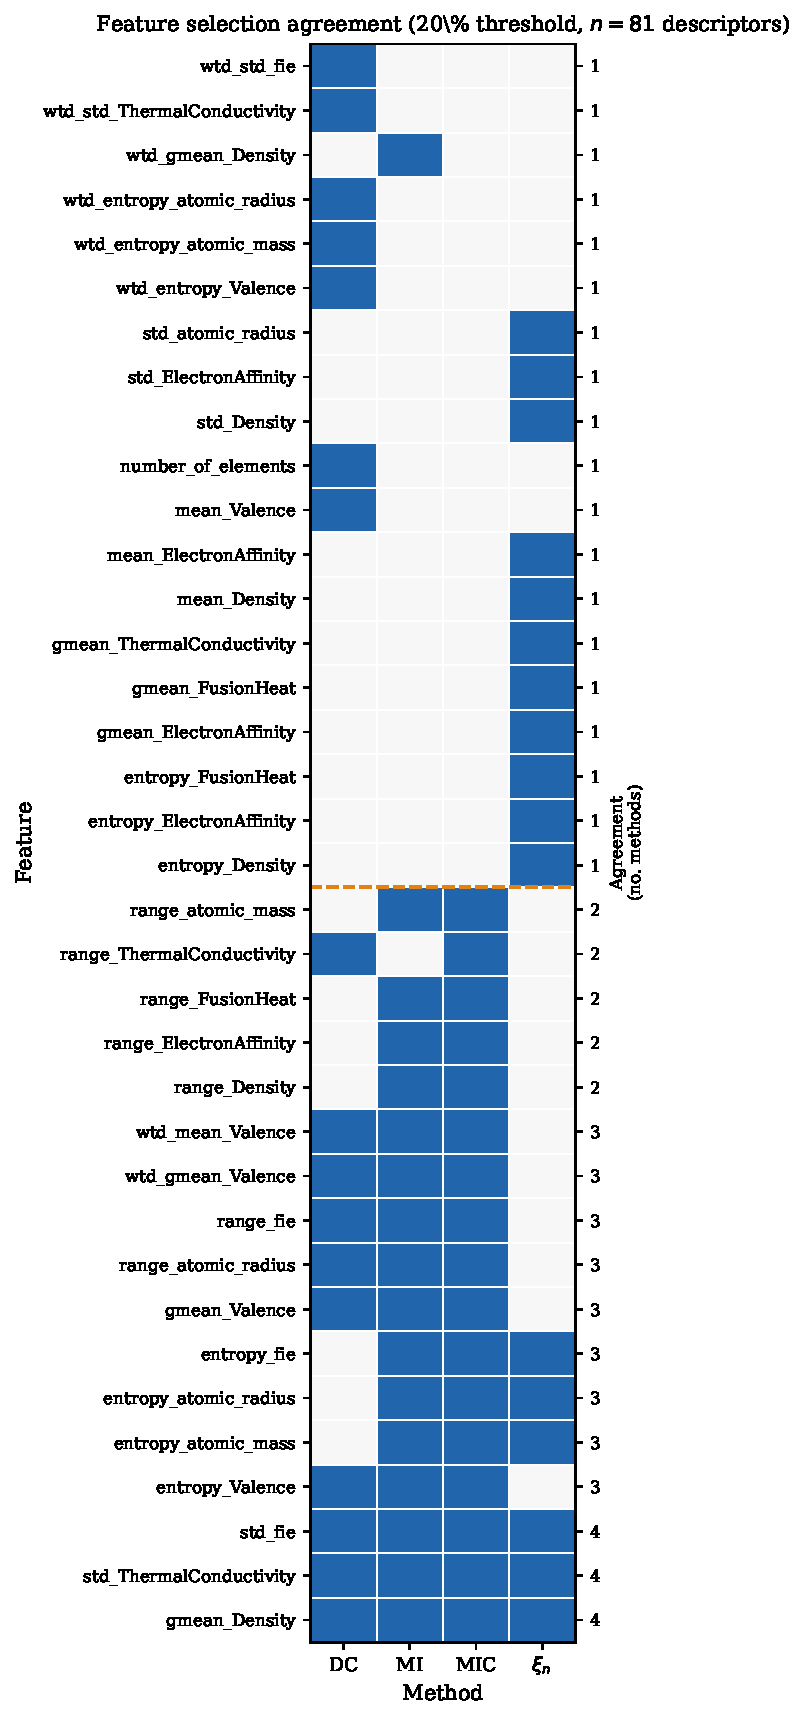
\includegraphics[width=\columnwidth]{feature_agreement_matrix}
\caption{Feature selection agreement across the four dependence measures at the
20\% retention threshold, restricted to the 18 descriptors selected by two or
more methods ($p = 81$, $n = 15{,}542$). Rows are ordered by decreasing
agreement level (right axis). The complete 34-feature matrix, including the 13
single-method-only descriptors, is provided in
Appendix~\ref{app:feature_matrix}.}
\label{fig:agreement}
\end{figure}

\subsection{Stability Analysis: 30-Repetition Experiments}
\label{sec:stability}
We evaluate stability using 30 independent resampling runs with LightGBM at the 20\% feature retention threshold. Table~\ref{tab:stability_results} reports mean predictive performance, variability metrics, and feature selection stability across methods. 

DC achieves the highest mean
$R^2 = 0.893$, followed by MI and MIC (both ${\approx}\,0.877$), then $\xi_n$
($0.839$). The $0.054$-unit $R^2$ gap between DC and $\xi_n$ represents 6\%
relative to the mean of DC. All methods show a low coefficient of variation
(0.8\%--1.1\%), indicating highly reproducible performance under resampling.
The Jaccard similarity exceeds 0.94 for every method, implying that selected
feature sets overlap by at least 94\% across repetitions. MIC requires
approximately $30\times$ more total pipeline time than $\xi_n$
(191.5~min versus 6.5~min) while achieving similar stability. The standard
deviations of $0.007$--$0.010$ in $R^2$ confirm consistent performance across
random splits, validating the experimental protocol.

\begin{table}[t]
\centering
\caption{Stability metrics from 30 independent repetitions
(LightGBM, 20\% threshold).}
\label{tab:stability_results}
\small
\begin{tabular}{lccccc}
\toprule
Method & $R^2$ (mean $\pm$ std) & RMSE (K) & CoV($R^2$) & Jaccard Similarity
  & Time (min) \\
\midrule
DC      & $\mathbf{0.893 \pm 0.010}$ & $\mathbf{11.04 \pm 0.54}$ & 1.1\%
  & $0.94 \pm 0.06$ & \phantom{0}7.0 \\
MI      & $\underline{0.877 \pm 0.008}$ & $\underline{11.83 \pm 0.42}$ & 0.9\%
  & $0.94 \pm 0.06$ & \phantom{0}9.8 \\
MIC     & $0.877 \pm 0.007$ & $11.84 \pm 0.37$ & \textbf{0.8\%}
  & $\mathbf{0.96 \pm 0.06}$ & 191.5 \\
$\xi_n$ & $0.839 \pm 0.007$ & $13.54 \pm 0.31$ & \underline{0.9\%}
  & $\underline{0.95 \pm 0.06}$ & \phantom{0}\underline{6.5} \\
\bottomrule
\end{tabular}
\smallskip\\
{\small\textit{Note.} Bold indicates best result per column; underline indicates
second best. CoV: coefficient of variation; Time: total pipeline time including
hyperparameter tuning and model training. Pairwise paired effect sizes
(Cohen's $d_z$) computed on the same 30 shared splits, with mean differences
in $R^{2}$ units and 95\% BCa bootstrap intervals, are summarized in the
paragraph below and deposited in full at
\texttt{results/stability/cohens\_d\_\{pairwise,matrix\_r2,matrix\_mae\}.csv}
in the accompanying repository.}
\end{table}

Pairwise paired effect sizes on the $R^{2}$ metric corroborate and refine the
per-method summaries in Table~\ref{tab:stability_results}. Because the four
measures are evaluated on identical resampling splits, Cohen's
$d_z = \bar{\Delta} / s_{\Delta}$ ($n = 30$ paired splits;
\citealt{Cohen1988, Lakens2013}) characterizes the consistency of
per-split rank-order rather than its absolute spread. The three contrasts
involving $\xi_n$ are uniformly directional with $\xi_n$ dominated by every
symmetric measure ($d_z = 9.3$--$10.9$ for DC--$\xi_n$, MI--$\xi_n$, and
MIC--$\xi_n$), reflecting the $\bar{\Delta} = 0.038$--$0.054$ $R^{2}$ gap
between $\xi_n$ and each of the three symmetric measures together with
within-pair standard deviations $s_{\Delta} \approx 0.004$--$0.006$. DC
similarly dominates both MI and MIC ($d_z \approx 4.9$;
$\bar{\Delta} \approx 0.016$ $R^{2}$), while MI and MIC are
indistinguishable on this metric ($d_z = 0.06$; BCa interval crossing zero).
The MAE-based sensitivity analysis agrees in direction across all six
contrasts. We emphasize that these magnitudes derive from a within-subjects
design with tightly constrained $s_{\Delta}$ and are not interpretable on
the between-subjects $d$ scale of Figure~\ref{fig:stat_tests}b; the relevant
absolute-scale anchors are the $\bar{\Delta}$ values in $R^{2}$ units and the
BCa intervals reported in the accompanying CSVs. Accordingly, statistical
separation under repeated resampling should be interpreted jointly with the
absolute $\bar{\Delta}$ values, stability metrics, and computational
trade-offs rather than from standardized effect magnitudes alone.

The generalization gap $\Delta R^{2}$ is smallest for $\xi_n$
($0.031 \pm 0.007$) compared to DC ($0.058 \pm 0.011$),
MI ($0.045 \pm 0.009$), and MIC ($0.042 \pm 0.008$). This confirms superior
generalization stability for $\xi_n$, independent of its absolute predictive
performance. DC and $\xi_n$ occupy opposing vertices of the non-dominated
frontier shown in Figure~\ref{fig:pareto}. Table~\ref{tab:bootstrap_cv}
quantifies this accuracy--stability tension across all configurations.

\begin{figure}[t]
\centering
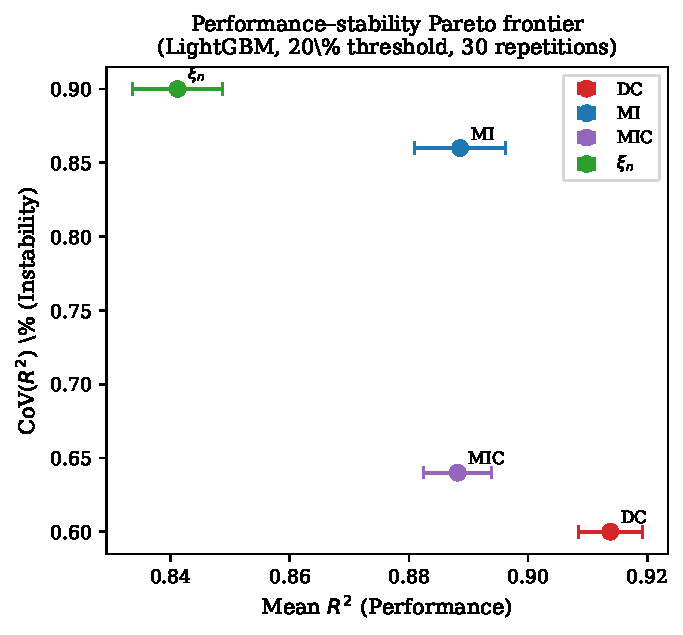
\includegraphics[width=0.9\linewidth]{fig3_pareto}
\caption{Performance--stability Pareto frontier for the four dependence measures
(LightGBM, 20\% threshold, 30 repetitions). Higher mean $R^2$ is better
(right); lower CoV is better (down). The shaded region marks the
Pareto-optimal zone.}
\label{fig:pareto}
\end{figure}

\begin{table}[t]
\centering
\caption{Bootstrap stability metrics across feature selection methods.}
\label{tab:bootstrap_cv}
\begin{tabular}{lcccc}
\toprule
Method & CoV($R^2$) & CoV(RMSE) & CoV(MAE) & Train--Test Gap \\
\midrule
$\xi_n$ & \textbf{17.25\%} & \textbf{19.82\%} & \textbf{24.56\%}
  & $\mathbf{0.031 \pm 0.007}$ \\
DC      & 19.33\% & 22.15\% & 30.37\% & $0.058 \pm 0.011$ \\
MI      & 24.78\% & 26.42\% & 28.28\% & $0.045 \pm 0.009$ \\
MIC     & 21.45\% & 23.89\% & 27.13\% & $0.042 \pm 0.008$ \\
\bottomrule
\end{tabular}
\smallskip\\
{\small\textit{Note.} Bold indicates lowest (most favorable) value per column.}
\end{table}

This stability differential has two practical implications. First, $\xi_n$
selections remain consistent under data perturbation, potentially improving
reproducibility across independent evaluations. Second, the narrower
generalization gap ($\Delta R^{2} = 0.031 \pm 0.007$ versus
$0.058 \pm 0.011$ for DC) indicates that $\xi_n$-selected subsets are less
prone to overfitting in downstream modeling.

\subsection{Practical Significance in Materials Discovery}
\label{sec:practical}
The gap of $0.054$~$R^2$ between DC and $\xi_n$ corresponds to approximately
2.5~K in RMSE (11.04~K versus 13.54~K). At liquid nitrogen temperature
(77~K), this represents a relative error reduction of 3.2\%. This is
significant for high-throughput screening where experimental validation costs
\$10,000--\$100,000 per candidate material. However, $\xi_n$'s 95\%
computational advantage over MIC becomes practically decisive in production
pipelines processing thousands of materials daily.

Table~\ref{tab:feature_selection_timing} isolates the computational cost of the
feature selection step. $\xi_n$ is $5.6\times$ faster than DC and
$1{,}412\times$ faster than MIC ($0.33$~s versus $465.99$~s) for a single
scoring pass. The timing differences in Table~\ref{tab:stability_results}
therefore stem primarily from the correlation computation, not from the
subsequent modeling steps.

\begin{table}[t]
\centering
\begin{threeparttable}
\caption{Computational efficiency of feature selection methods (isolated scoring
step).}
\label{tab:feature_selection_timing}
\begin{tabular}{lcccc}
\toprule
Method & Mean Time (s) & Std (s) & Time per Feature (ms) & Speedup vs.\ DC \\
\midrule
$\xi_n$ & \textbf{0.33} & 0.05 & \phantom{0}4.0 & $5.6\times$ \\
DC      & \underline{1.83} & 0.08 & \phantom{0}22.6 & $1.0\times$ (baseline) \\
MI      & 7.30 & 0.56 & \phantom{0}90.1 & $0.25\times$ \\
MIC     & 465.99 & 19.12 & 5753.0 & $0.004\times$ \\
\bottomrule
\end{tabular}
\begin{tablenotes}
\item[]\footnotesize \textit{Note.} Single-pass feature selection timing on
$n = 15{,}542$ samples and $p = 81$ features, averaged over 30 independent
repetitions. MIC was computed using \texttt{minepy==1.2.6}
\citep{Albanese2013minepy} (Python~3.10, isolated conda environment);
$\xi_n$, MI, and DC were computed in the main pipeline environment.
Time per feature is mean time divided by 81. Speedup is relative to DC.
Total pipeline time, including hyperparameter tuning and model training,
is reported in Table~\ref{tab:stability_results}.
\end{tablenotes}
\end{threeparttable}
\end{table}

\subsection{Interpretation of High Intra-Method Stability}
The intra-method stability ($J_{\mathrm{stab}} = 0.94$--$0.96$;
Table~\ref{tab:stability_results}) measures how consistently a single method
re-selects the same features across 30 independent resamples. This quantity is
conceptually distinct from the inter-method agreement in a fixed split
($J_{\mathrm{agree}}$), which quantifies overlap between methods and is
visualized in Figure~\ref{fig:agreement}. The high $J_{\mathrm{stab}}$ values
are consistent with the feature-engineering structure of the dataset. With 81
descriptors derived from only 8 base atomic properties, the top-ranked features
under any measure are drawn from a narrow dominant-predictor pool. Three
structural factors reinforce this: (1)~the 81 descriptors derive from 8 base
properties, creating natural feature families from which all methods tend to
select representatives; (2)~certain features such as weighted-mean atomic mass
and valence-related descriptors consistently exhibit strong correlations with
$T_c$ under all measures; and (3)~at the 20\% threshold, selecting 16 of 81
features isolates the strongest predictors on which all methods converge.

The asymmetric nature of $\xi_n$ manifests in subtle ranking differences at the
margin. All methods agree on \emph{which} features are important but disagree
on their \emph{relative importance} at the threshold boundary. These marginal
ranking differences, rather than general disagreement about dominant predictors,
explain why $\xi_n$ achieves 94\% of DC's performance despite high
$J_{\mathrm{stab}}$.

\subsection{Scalability Implications}
$\xi_n$ demonstrates a $1{,}412\times$ speed advantage over MIC
(Table~\ref{tab:feature_selection_timing}). However, the moderate scale of this
dataset ($n = 15{,}542$, $p = 81$) may not reveal regimes in which
computational efficiency dominates accuracy trade-offs. The crossover point at
which $\xi_n$'s $\mathcal{O}(n \log n)$ advantage over DC's $\mathcal{O}(n^2)$
becomes practically decisive depends on the $(n,\, p)$ scaling regime and
domain-specific correlation structure. Generalization to datasets with
$p \gg 81$ or $n \gg 10^5$, such as genome-wide association panels or financial
time series, cannot be assumed from the present results. The empirical
complexity crossover for $n \in [15{,}542,\, \infty)$ remains an open
scientific question.

\subsection{Method Selection Guidelines}
Table~\ref{tab:select} provides practical guidance derived from experimental
evidence. Choose $\xi_n$ when computational efficiency is paramount and a 6\%
accuracy sacrifice is acceptable. Choose DC for maximum accuracy. Choose MIC
when stability documentation is required despite its computational cost.

\newcolumntype{L}{>{\raggedright\arraybackslash}p{0.42\linewidth}}
\newcolumntype{R}{>{\raggedright\arraybackslash}p{0.50\linewidth}}
\begin{table}[t]
\centering
\caption{Recommended dependence measure by research context.}
\label{tab:select}
\begin{tabular}{LR}
\toprule
Research context & Recommended method \\
\midrule
One-time analysis, accuracy paramount &
  DC (highest $R^{2} = 0.893$ $\pm 0.010$) \\
High-throughput screening, speed required &
  $\xi_n$ (6.5~min; 94\% of DC accuracy) \\
Reproducibility-critical analysis, stability paramount &
  MIC (lowest CoV: 0.8\%; Jaccard: 0.96) \\
Exploratory, balanced approach &
  MI (second in accuracy and speed) \\
Budget constraints, large scale &
  $\xi_n$ ($30\times$ faster than MIC) \\
Ensemble strategy &
  DC $+$ $\xi_n$ (complementary asymmetry) \\
\bottomrule
\end{tabular}
\end{table}

%%%%%%%%%%%%%%%%%%%%%%%%%%%%%%%%%%%%%%%%%%%%%%%%%%%%%%%%%%
\section{Discussion}
%%%%%%%%%%%%%%%%%%%%%%%%%%%%%%%%%%%%%%%%%%%%%%%%%%%%%%%%%%
The results demonstrate that dependence measures exhibit systematic differences
not only in predictive accuracy but also in stability and robustness,
necessitating a multi-criteria evaluation framework. The Friedman test
($\chi^{2} = 27.9$, $p < 0.001$; Table~\ref{tab:overall_results}) confirms
that these differences are statistically significant, yet the negligible-to-small
Cohen's $d$ effect sizes ($|d| = 0.09$--$0.33$; Figure~\ref{fig:stat_tests})
indicate that the hierarchy is driven primarily by threshold-induced variance in
ranking at the feature margin rather than fundamental differences in ranking
quality. This distinction is critical: it suggests that method choice matters
less for the dominant predictor pool than for the borderline descriptors that
determine the effective $R^2$ ceiling of each filter.

A key finding is that $\xi_n$, despite its theoretical advantages, does not
achieve the highest predictive accuracy in this setting ($R^2 = 0.839$ versus
DC's $0.893$; Table~\ref{tab:stability_results}). This is consistent with the
mechanistic argument that symmetric dependence measures such as DC capture
bidirectional relationships among borderline descriptors that asymmetric
$Y \mid X$ scoring systematically underweights. DC's preferential retention of
these high-impact borderline features explains its $R^2$ advantage and is
directly evidenced by the 7 $\xi_n$-exclusive descriptors (range 6--8) in
Figure~\ref{fig:agreement} that no symmetric measure selects. However, the
asymmetric and rank-based construction of $\xi_n$ offers distinct advantages
for feature selection: by aligning directly with the objective of ranking
predictors with respect to a response variable, it provides a more
interpretable and stable selection mechanism, particularly under
multicollinearity.

The observed accuracy--stability trade-off (Figure~\ref{fig:pareto}) highlights
a fundamental tension in filter-based feature selection: methods that maximize
predictive performance may not yield maximally reproducible feature sets.
$\xi_n$ occupies the low-accuracy, low-variance vertex of this frontier, with
the smallest generalization gap ($\Delta R^2 = 0.031 \pm 0.007$;
Table~\ref{tab:bootstrap_cv}) and a competitive Jaccard stability of
$0.95 \pm 0.06$ (Table~\ref{tab:stability_results}), comparable to MIC's
$0.96 \pm 0.06$ despite being $1{,}412\times$ faster
(Table~\ref{tab:feature_selection_timing}). This underscores the importance of
evaluating feature selection methods under multiple criteria simultaneously,
as single-metric comparisons obscure trade-offs that are consequential for
scientific reproducibility and production deployment.

%%%%%%%%%%%%%%%%%%%%%%%%%%%%%%%%%%%%%%%%%%%%%%%%%%%%%%%%%%
\section{Limitations}
%%%%%%%%%%%%%%%%%%%%%%%%%%%%%%%%%%%%%%%%%%%%%%%%%%%%%%%%%%
The present evaluation is conducted on a single materials-science dataset.
This reflects a deliberate methodological choice: characterising the
accuracy--stability--cost trade-off surface requires holding the data
structure $(n,\, p,\, \rho)$ constant so that observed differences are
attributable to the ranking quality of each dependence measure rather than
to dataset-specific correlation structure. The 30-repetition resampling
design provides within-dataset evidence that the identified trade-offs are
stable under sampling variability; it does not address cross-domain
transferability.

The dataset employed here exhibits a specific structural regime:
$n = 15{,}542$, $p = 81$, with high multicollinearity (condition index
$> 30$ in 52\% of features) and dense outlier prevalence (82.7\% of
descriptors). Findings are most directly applicable to datasets with
similar $(n,\, p)$ structure and comparable dependence regimes.
Generalisation to high-dimensional settings ($p \gg n$), sparse data, or
time-series dependence cannot be assumed from the present results.

These questions are addressed in a companion study \citep{ngorima2026complexity} that
applies the same pipeline to a genomics dataset
($n = 10{,}967$, $p = 20{,}531$; TCGA PANCAN) and a macroeconomic panel
(FRED-MD), representing structurally distinct $(n,\, p)$ regimes. Together,
KsaaiP1 and KsaaiP2 provide complementary evidence: controlled depth on a
well-characterised benchmark, and cross-domain breadth across regimes in
which computational and ranking properties differ qualitatively.

The study is further restricted to fixed retention thresholds
($\alpha \in \{10\%, 20\%, 30\%\}$). Adaptive threshold selection and
wrapper-based methods lie outside the present scope.
Full pipeline reproducibility requires an isolated Python~3.10 environment
for \texttt{minepy}; archived MIC results are provided for users on
Python~3.12 (see Code and Data Availability).

%%%%%%%%%%%%%%%%%%%%%%%%%%%%%%%%%%%%%%%%%%%%%%%%%%%%%%%%%%
\section{Conclusion}
%%%%%%%%%%%%%%%%%%%%%%%%%%%%%%%%%%%%%%%%%%%%%%%%%%%%%%%%%%
\section{Conclusion}

We presented a cmparative benchmark of Chatterjee's $\xi_n$ against established dependence measures (DC, MI, MIC) across 48 feature-selection configurations and 30 repeated resampling runs on a superconductivity dataset ($n = 15{,}542$, $p = 81$).

Across all settings, DC achieved the highest predictive performance ($R^{2} = 0.893 \pm 0.010$), while $\xi_n$ achieved approximately 94\% of this performance with reduced computational cost and faster per-step scoring time. All methods exhibited high stability under repeated resampling, with Jaccard similarity between 0.94 and 0.96 and low coefficients of variation (0.8\%--1.1\%).

Nonparametric Friedman testing indicated statistically significant differences in ranking across methods, with a consistent ordering of DC $\succ$ MI $\approx$ MIC $\succ$ $\xi_n$ ($p < 0.001$). Post-hoc comparisons confirmed pairwise rank separations for key contrasts. Effect size analysis using Cohen's $d_z$ and BCa bootstrap confidence intervals indicated that observed differences are small in standardized magnitude but stable across resampling.

From a computational perspective, $\xi_n$ provides a consistent speed advantage over MIC and a moderate efficiency gain relative to DC, while maintaining competitive predictive performance. The observed $R^{2}$ difference between DC and $\xi_n$ corresponds to a 2.5~K RMSE gap in this dataset.

Overall, the results highlight a trade-off between predictive accuracy, computational cost, and stability across dependence measures. $\xi_n$ occupies a computationally efficient regime, making it suitable for high-throughput screening settings where moderate reductions in predictive accuracy are acceptable. DC remains preferable when maximum predictive accuracy is required.

The study contributes (i) a controlled comparative evaluation of $\xi_n$, (ii) a multi-repetition benchmarking protocol across 48 configurations, (iii) evidence of high reproducibility across modern dependence measures, and (iv) practical guidance for method selection under different computational constraints. Generalization to substantially larger or structurally different datasets remains an open empirical question.

\acks{This work extends the author's MSc thesis completed at the University of
Stirling, UK (supervised by Professor Kevin Swingler). Experiments use the
publicly available Hamidieh--Matasov superconductivity dataset
\citep{Hamidieh2018data, Matasov2020vis}. Computational implementations rely on
scikit-learn \citep{Pedregosa2011scikit}, LightGBM \citep{Ke2017lightgbm},
Optuna \citep{Akiba2019optuna}, \texttt{xicor} \citep{xicor2021}, and
\texttt{minepy} \citep{Albanese2013minepy}.
The author declares no funding and no competing interests.}

\newpage

\appendix
%%%%%%%%%%%%%%%%%%%%%%%%%%%%%%%%%%%%%%%%%%%%%%%%%%%%%%%%%%
\section{Complete Feature Agreement Matrix}
\label{app:feature_matrix}
%%%%%%%%%%%%%%%%%%%%%%%%%%%%%%%%%%%%%%%%%%%%%%%%%%%%%%%%%%
Figure~\ref{fig:agreement_full} presents the full binary agreement matrix for
all 34 descriptors appearing in at least one selected subset at the 20\%
retention threshold. The 13 single-method-only descriptors (agreement level~1)
are retained here for completeness but excluded from the main-text
Figure~\ref{fig:agreement}, which focuses on the 18 analytically informative
consensus features (agreement $\geq 2$).
 
\begin{figure}[htb]
\centering
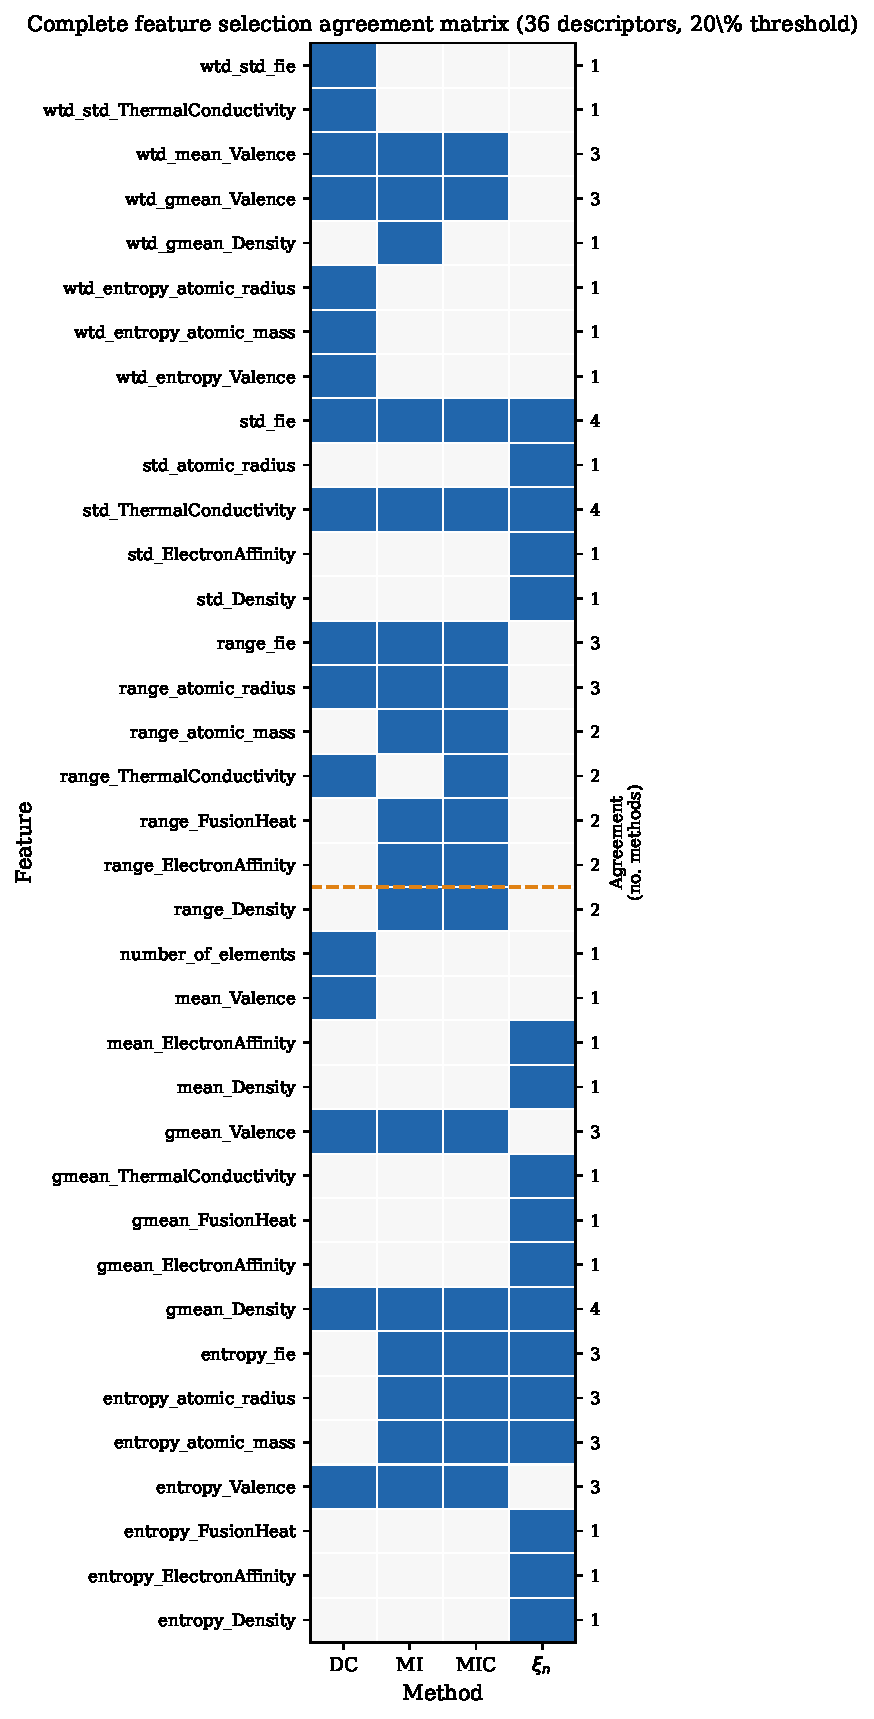
\includegraphics[width=\columnwidth]{full_feature_agreement_matrix}
\caption{Complete feature selection agreement matrix for all 34 descriptors
selected by at least one method at the 20\% retention threshold
($p = 81$, $n = 15{,}542$). Rows are ordered by decreasing agreement level
(right axis). The dashed horizontal rule separates features with agreement
$\geq 2$ (upper panel, reproduced as Figure~\ref{fig:agreement} in the main
text) from single-method-only descriptors (lower panel).}
\label{fig:agreement_full}
\end{figure}

%%%%%%%%%%%%%%%%%%%%%%%%%%%%%%%%%%%%%%%%%%%%%%%%%%%%%%%%%%
\section{Hyperparameter Search Spaces}
\label{app:hyperparams}
%%%%%%%%%%%%%%%%%%%%%%%%%%%%%%%%%%%%%%%%%%%%%%%%%%%%%%%%%%
Table~\ref{tab:hyperparams} reports the hyperparameter search bounds used in
Optuna Bayesian optimization for all four model classes. Lasso and Elastic Net
used 50 trials in Experiment~1 and 20 trials in Experiment~2. LightGBM and
Random Forest used the same trial counts respectively.

\begin{table}[t]
\centering
\caption{Hyperparameter search spaces for Bayesian optimization (Optuna).}
\label{tab:hyperparams}
\begin{tabular}{llll}
\toprule
Model & Parameter & Type & Range \\
\midrule
Lasso         & $\alpha$              & log-uniform & $[10^{-4},\ 10^{2}]$ \\
Elastic Net   & $\alpha$              & log-uniform & $[10^{-4},\ 10^{2}]$ \\
              & $\ell_1$ ratio        & uniform     & $[0.1,\ 0.9]$ \\
LightGBM      & num\_leaves           & integer     & $[20,\ 300]$ \\
              & learning\_rate        & log-uniform & $[10^{-3},\ 0.3]$ \\
              & n\_estimators         & integer     & $[100,\ 1000]$ \\
              & min\_child\_samples   & integer     & $[5,\ 100]$ \\
Random Forest & n\_estimators         & integer     & $[100,\ 1000]$ \\
              & max\_depth            & integer     & $[3,\ 20]$ \\
              & min\_samples\_split   & integer     & $[2,\ 20]$ \\
\bottomrule
\end{tabular}
\end{table}

%%%%%%%%%%%%%%%%%%%%%%%%%%%%%%%%%%%%%%%%%%%%%%%%%%%%%%%%%%
\section{Code and Data Availability}
\label{app:data}
%%%%%%%%%%%%%%%%%%%%%%%%%%%%%%%%%%%%%%%%%%%%%%%%%%%%%%%%%%
This study uses the curated superconductivity dataset of \citet{Matasov2020vis},
derived from the original measurements of \citet{Hamidieh2018data}. The file
\texttt{sc\_mean.csv} is publicly available at
\url{https://github.com/matasovav/DATA_SC/blob/master/sc_mean.csv}.
The full experimental pipeline, including all preprocessing, feature selection,
model training, and evaluation scripts, is publicly available at
\url{https://github.com/TinasheNgorima/ksaai-feature-selection-benchmark}
and permanently archived at \url{https://doi.org/10.5281/zenodo.19675804}
\citep{ngorima2026ksaai}.
$\xi_n$ scores were computed using \texttt{xicor} \citep{xicor2021}. MIC
scores were computed using \texttt{minepy==1.2.6} \citep{Albanese2013minepy}
in an isolated conda environment (Python~3.10), as \texttt{minepy} requires a
build toolchain incompatible with Python~3.12. The remaining three methods
($\xi_n$, MI, DC) are fully reproducible from the public repository on
Python~3.12. Original MIC results from the manuscript are archived in
\texttt{results/original\_run/} in the repository.

\vskip 0.2in
\bibliography{bibitem}

\end{document}